% Original moonlit city illustration; all shapes are editable TikZ paths.
% Copyright (C) 2026 Xiao Fan <xiaofan140@gmail.com>
% SPDX-License-Identifier: GPL-3.0-or-later
\documentclass[tikz,border=0pt]{standalone}
\definecolor{brand}{HTML}{7AA2F7}
\definecolor{sky}{HTML}{545C7E}
\definecolor{distant}{HTML}{414868}
\definecolor{city}{HTML}{343B58}
\definecolor{foreground}{HTML}{292E42}
\definecolor{violet}{HTML}{BB9AF7}
\definecolor{moon}{HTML}{C0CAF5}
\definecolor{light}{HTML}{E0AF68}
\begin{document}
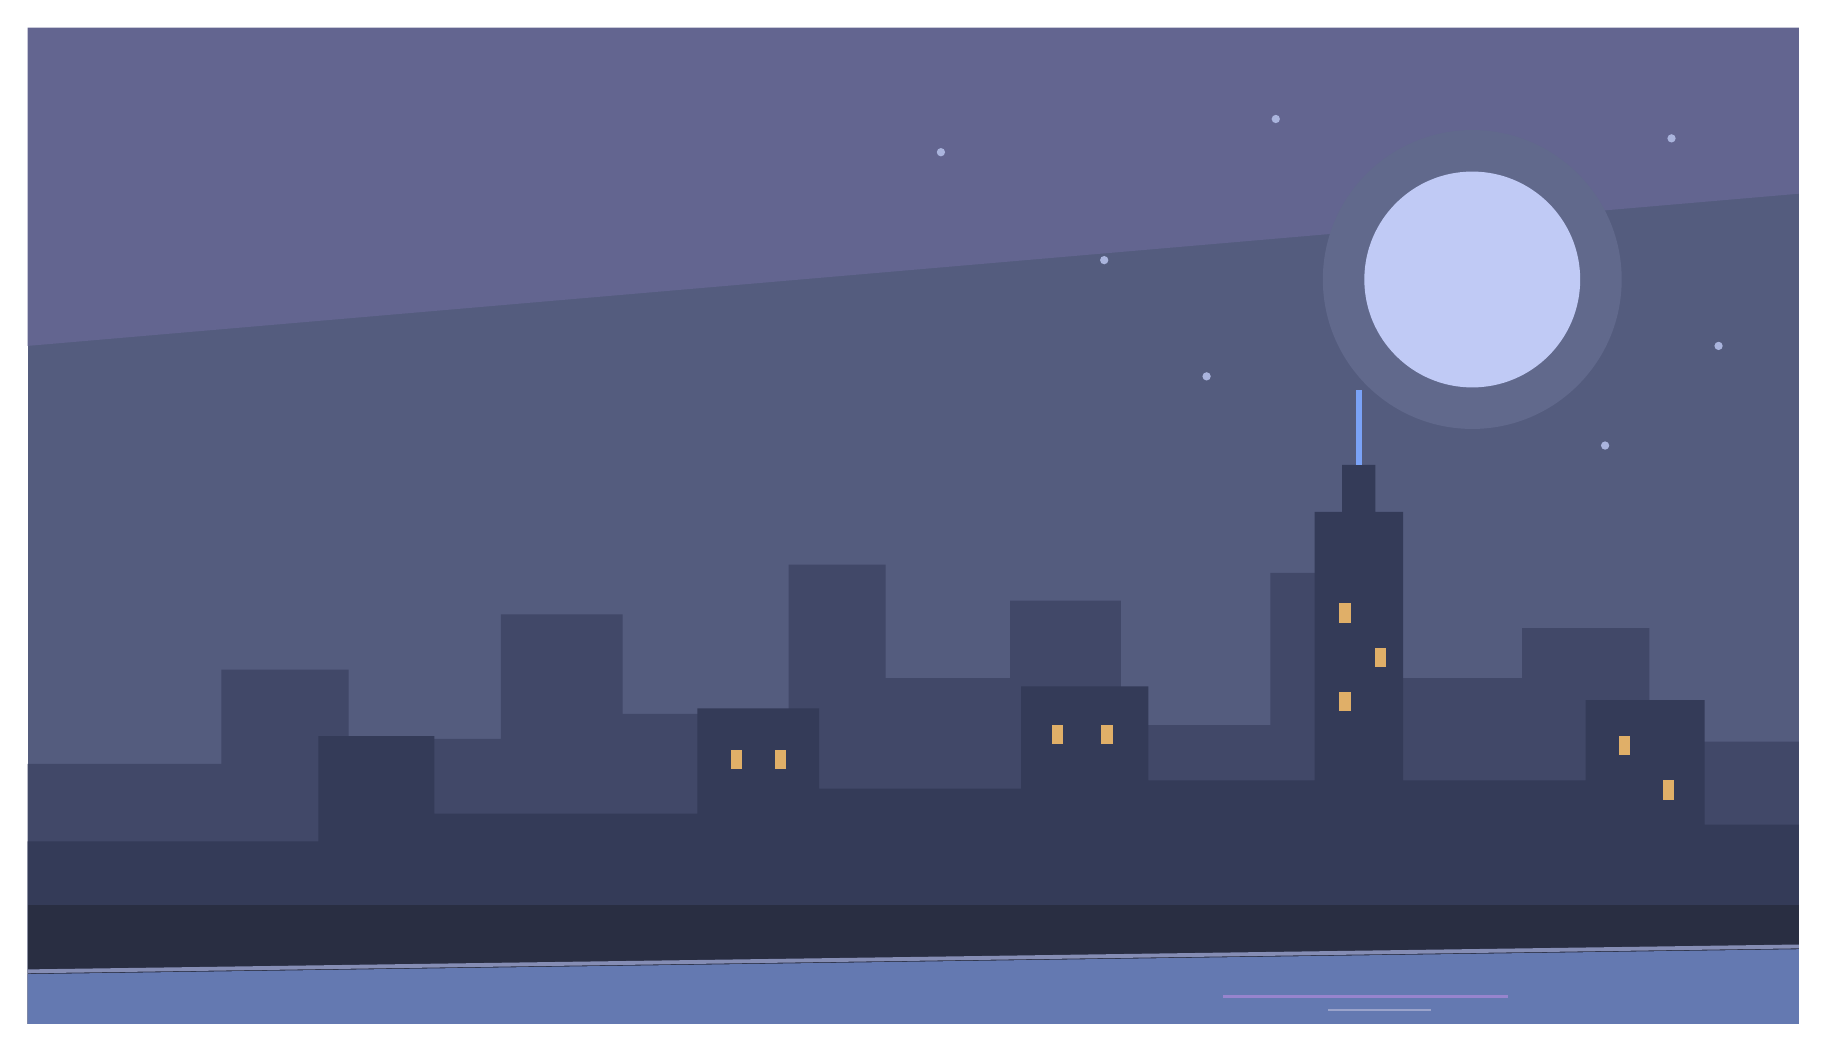
\begin{tikzpicture}[x=1pt,y=1pt]
  \clip (0,0) rectangle (640,360);
  % A lighter sky gives the shared diagonal mask a visible edge at the top.
  \fill[sky] (0,0) rectangle (640,360);
  \fill[violet!15!sky] (0,245) -- (640,300) -- (640,360) -- (0,360) -- cycle;
  \fill[moon!12!sky] (522,269) circle (54);
  \fill[moon] (522,269) circle (39);
  \foreach \x/\y in {330/315,389/276,451/327,594/320,611/245,426/234,570/209}{
    \fill[moon!80!sky] (\x,\y) circle (1.5);
  }
  % Three city layers; deliberately abstract rather than an identifiable building.
  \fill[distant] (0,0) -- (0,94) -- (70,94) -- (70,128) -- (116,128)
    -- (116,103) -- (171,103) -- (171,148) -- (215,148) -- (215,112)
    -- (275,112) -- (275,166) -- (310,166) -- (310,125) -- (355,125)
    -- (355,153) -- (395,153) -- (395,108) -- (449,108) -- (449,163)
    -- (484,163) -- (484,125) -- (540,125) -- (540,143) -- (586,143)
    -- (586,102) -- (640,102) -- (640,0) -- cycle;
  \fill[city] (0,0) -- (0,66) -- (105,66) -- (105,104) -- (147,104)
    -- (147,76) -- (242,76) -- (242,114) -- (286,114) -- (286,85)
    -- (359,85) -- (359,122) -- (405,122) -- (405,88) -- (465,88)
    -- (465,185) -- (475,185) -- (475,202) -- (487,202) -- (487,185)
    -- (497,185) -- (497,88) -- (563,88) -- (563,117) -- (606,117)
    -- (606,72) -- (640,72) -- (640,0) -- cycle;
  \draw[brand,line width=2] (481,202) -- (481,229);
  \foreach \x/\y in {254/92,270/92,370/101,388/101,474/145,487/129,474/113,575/97,591/81}{
    \fill[light] (\x,\y) rectangle +(4,7);
  }
  \fill[foreground] (0,0) rectangle (640,43);
  % A pale waterfront keeps the diagonal visible at its bottom as well.
  \fill[brand!42!sky] (0,0) -- (640,0) -- (640,27) -- (0,18) -- cycle;
  \draw[moon!45!sky,line width=1.4] (0,19) -- (640,28);
  \draw[violet!65!sky,line width=1] (432,10) -- (535,10);
  \draw[moon!65!sky,line width=1] (470,5) -- (507,5);
\end{tikzpicture}
\end{document}
